\documentclass[a4paper]{article}
\usepackage[utf8]{inputenc}
\usepackage{color}
\usepackage{url}
\usepackage[utf8]{inputenc}
\usepackage{graphicx}
\usepackage[english,serbian]{babel}
\usepackage[unicode]{hyperref}
\hypersetup{colorlinks,citecolor=green,filecolor=green,linkcolor=blue,urlcolor=blue}

\begin{document}

\title{Džonatan Bouen\\ \small{Seminarksi rad u okviru kursa\\Tehničko i naučno pisanje\\Matematički fakultet}}

\author{Vladimir Jovanović\\vlad.jov.096@gmail.com}
\maketitle

\abstract{\textbf{Džonatan P. Bouen} (rođen 1956. godine) je britanski stručnjak za računare.}

\tableofcontents
\newpage

\begin{tabular}{|l|l|}

\hline
\multicolumn{2}{|c|}{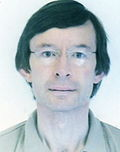
\includegraphics[scale=6]{Jonathan_Bowen_photograph.jpg}} \\
\hline
\textbf{Datum rođenja} & 1956.\\
\hline
\textbf{Mesto rođenja} & Oksford, Ujedinjeno Kraljevstvo\\
\hline
\textbf{Prebivalište} & Oksford\\
\hline
\textbf{Državljanstvo} & Ujedinjeno Kraljevstvo\\
\hline
\textbf{Škola} & Univerzitetski koledž (Oksford)\\
\hline
\multicolumn{2}{|c|}{\textbf{Naučna karijera}} \\
\hline
\textbf{Polje} & Informatika \\ 
& Informaciona tehnologija \\ 
& Muzejska informatika\\
\hline
\textbf{Institucije} & \textit{Museophile Limited}\\
& Univerzitet u Birmingemu\\
& Univerzitet u Redingu\\
& Univerzitet u Oksfordu\\
& \textit{London South Bank} univerzitet\\
& Imperijal Koledž, London\\
\hline
\textbf{Poznat po} & Formalne metode\\
& \textit{Z-notacija}\\
& Stranice muzeja virtuelne biblioteke\\
& Virtuelni muzej računarstva\\
\hline
\textbf{Uticaji} & Dejvid Berman\\
& Džek Kouplend\\
& Majk Gordon\\
& Džejms Hemzli\\
& Toni Hor\\
& Klif Džouns\\
& Alan Tjuring\\
\hline
\textbf{Uticao na} & Majk Hinči\\
& Kevin Lano\\
\hline

\end{tabular}

\newpage
\section{Pregled}
\label{sec:pregled}
Džonatan Bouen je predstavnik „Museophile Limited” kompanije i profesor emeritus na London South Bank univerzitetu, gde je rukovodio Centrom za primenjene formalne metode. Bio je profesor računarske nauke na Univerzitetu u Birmingemu, gostujući profesor na institutu Prat (Njujork), Univerziteta u Vestminsteru, Kings koledža (London), i gostujući akademik na Londonskom univerzitetskom koledžu.

\section{Obrazovanje}
Rođen je u Okfsordu, sin Hamfrija Bouena, a školovao se u tzv. „Dragon School” (Oksford) i u školi u Brajanstonu pre nego što je maturirao na Univerzitetskom koledžu u Oksfordu, gde je stekao zvanje magistra inžinjerskih nauka. 
\section{Karijera}
Bouen je kasnije radio na koledžu „Imperial College” u Londonu, kompjuterskoj laboratoriji univerziteta u Oksfordu (sada odseku za informatičke tehnologije na univerzitetu u Oksfordu), na Univerzitetu u Redingu i univerzitetu „London South Bank”. Njegov rani rad bio je zasnovan generalno na formalnim metodama, a kasnije naročito na „Z-notaciji” (engl. \textit{the Z notations}). Bio je predstavnik grupe „Z-korisnika” (engl. \textit{the Z user group}) od ranih 1990-ih godina do 2011. godine. Proglašen je predstavnikom britanskog kompjuterskog društva „FACS” (engl. \textit{Specialist Group on Formal Aspects of Computing Science}) 2002. godine. Od 2005. godine, Bouen je pomoćnik glavnog urednika novina „Inovacije u sistemu i softverskom inženjerstvu”. Pored toga, saradnik je i urednika naslovne strane novina „ACM Computing Surveys”, pokrivajući oblast softverskog inženjerstva i formalnih metoda. Od 2008.–2009. godine, bio je saradnik u „Praxis High Integrity Systems” i radio na velikom industrijskom projektu koristeći Z-notacije. 
\section{Odabrane knjige}

Izvor \cite{misc:1} se nalazi u tekstu. \\ 
Izvor \cite{misc:2} se nalazi u tekstu. \\
Izvor \cite{misc:3} se nalazi u tekstu.\\
Izvor \cite{misc:4} se nalazi u tekstu.\\
Izvor \cite{misc:5} se nalazi u tekstu.\\
Izvor \cite{misc:6} se nalazi u tekstu.\\
Izvor \cite{misc:7} se nalazi u tekstu.\\
Izvor \cite{misc:8} se nalazi u tekstu.\\
Izvor \cite{misc:9} se nalazi u tekstu.\\
Izvor \cite{book:1} se nalazi u tekstu.\\
Izvor \cite{book:2} se nalazi u tekstu.\\
Izvor \cite{aritcle:1} se nalazi u tekstu.\\
Izvor \cite{article:2} se nalazi u tekstu.\\
Izvor \cite{article:3} se nalazi u tekstu.\\
Izvor \cite{article:4} se nalazi u tekstu.\\

\bibliography{sources} 
\bibliographystyle{ieeetr}
\end{document}
